% !TEX encoding = UTF-8 Unicode
% \documentclass{article}
% \usepackage{../../superstyle}
% \usepackage{listings}
% \usepackage{amsmath}
% \begin{document}
% remove all before

%oppgavetekst
Oppgave tekst: 

Now repeat Step 4 with a more tightly grouped set of satellites. Choose all $\phi$$_i$ within
5 percent of one another and all $\theta$$_i$ within 5 percent of one another. Solve with and without the same input error as in Step 4. Find the maximum position error and error magnification factor. Compare the conditioning of the GPS problem when the satellites are tightly or loosely bunched.

\vspace{5mm}
Løsning

\begin{lstlisting}[caption={Task3.m}]
function [conditionNumber, worst_max_pos_error] = task5()

rho = 26570;

phi = [pi/4 (pi/4)*1.015 (pi/4)*1.03 (pi/4)*1.045];
theta = [pi pi*1.015 pi*1.030 pi*1.045];
A = ones(1,4); 
B = ones(1,4); 
C = ones(1,4);

for i=1:4
    A(i) = rho * cos(phi(i)) * cos(theta(i));
    B(i) = rho * cos(phi(i)) * sin(theta(i));
    C(i) = rho * sin(phi(i));
end

c = 299792.458;

R = sqrt((A.^2)+(B.^2)+((C-6370).^2));
t = 0.0001 + (R/c);

[x,y,z,d]= task2general(A,B,C,t); 
riktig = [x y z d];

factor = [[-1,-1,-1,-1];[1,1,1,1];[-1,-1,-1,1];[-1,-1,1,1];
		  [-1,1,1,1];[-1,1,-1,1];[-1,1,1,-1];[-1,-1,1,-1];
		  [-1,1,-1,-1];[1,1,1,-1];[1,1,-1,-1];[1,-1,-1,-1];
		  [1,-1,1,-1];[1,-1,-1,1];[1,1,-1,1];[1,-1,1,1]];

max_pos_error = zeros(1,16);
emf = zeros(1,16);

for i = 1:length(factor)
    dt1(1) = t(1) + 1e-8*factor(i,1);
    dt1(2) = t(2) + 1e-8*factor(i,2);
    dt1(3) = t(3) + 1e-8*factor(i,3);
    dt1(4) = t(4) + 1e-8*factor(i,4); 
    [x2,y2,z2,d2]=task2general(A,B,C,dt1);
    feil = [x2 y2 z2 d2];
    max_pos_error(i) = max(abs(riktig-feil));
    emf(i) = max_pos_error(i)/(c*max(abs(dt1-t)));
end

worst_max_pos_error = max(max_pos_error);
conditionNumber = max(emf);

end
\end{lstlisting}

\begin{figure}[h]
    \centering
    \includegraphics[width=0.9\textwidth]{sections/Exercise5/task5result}
    % \includegraphics[width=0.9\textwidth]{task5result}
    \caption{Matlabresultat fra oppgave 5}
    \label{fig:task5result}
\end{figure}

Som man ser i figur \ref{fig:task5result} er både kondisjonstallet og maksimum posisjonsfeil $\approx10^5$ høyere nå som alle satelittene er satt under 5\% fra hverandre i distanse kontra avstandene i exercise 4.

%tabeller
	\begin{figure}[h]
		\begin{minipage}{.5\textwidth}
			\centering
			\includegraphics[width=0.8\textwidth]{sections/Exercise5/emf.png}
			% \includegraphics[width=0.8\textwidth]{emf.png}
				\caption{Task 5 - EMF tabell}
				\label{fig:task5EMF}
		\end{minipage}
		\vspace{20 mm}
		\begin{minipage}{.5\textwidth}
			Felis porta sociis auctor amet ve eni scelerisque nonummy proin etiam. Curae purus dui. Massa magna quis eu nunc etiam porttitor egestas donec. Nulla porta risus proin diam ultrices torquent. Neque curae mollis ve purus in ipsum. Metus velit mauris lectus venenatis. Risus fusce leo. Ipsum felis. Fames lacus habitasse sed. Fames ipsum sit urna id sit auctor platea pede duis lacus habitant curabitur nisl ante. Netus dolor suspendisse et libero morbi sed placerat phasellus praesent cursus. Vitae velit dignissim dapibus aptent sociis class parturient duis nulla feugiat. Felis massa.
		\end{minipage}
		%\vspace{20 mm}

		\centering
	    \includegraphics[width=0.8\textwidth]{sections/Exercise5/emf_graph.png}
	    % \includegraphics[width=0.8\textwidth]{emf_graph.png}
		    \caption{Task 5 - EMF graf}
		    \label{fig:task5EMF_graph}
	\end{figure}

	\begin{figure}
		\begin{minipage}{.5\textwidth}
			\centering
			\includegraphics[width=0.8\textwidth]{sections/Exercise5/max_pos_error.png}
			% \includegraphics[width=0.8\textwidth]{max_pos_error.png}
		    	\caption{Task 5 - Maks. pos. tabell}
		    	\label{fig:task5max_pos_error}
		\end{minipage}
		\vspace{20 mm}
		\begin{minipage}{.5\textwidth}
			Felis porta sociis auctor amet ve eni scelerisque nonummy proin etiam. Curae purus dui. Massa magna quis eu nunc etiam porttitor egestas donec. Nulla porta risus proin diam ultrices torquent. Neque curae mollis ve purus in ipsum. Metus velit mauris lectus venenatis. Risus fusce leo. Ipsum felis. Fames lacus habitasse sed. Fames ipsum sit urna id sit auctor platea pede duis lacus habitant curabitur nisl ante. Netus dolor suspendisse et libero morbi sed placerat phasellus praesent cursus. Vitae velit dignissim dapibus aptent sociis class parturient duis nulla feugiat. Felis massa.
		\end{minipage}

		\centering
		\includegraphics[width=0.8\textwidth]{sections/Exercise5/max_pos_error_graph.png}
		% \includegraphics[width=0.8\textwidth]{max_pos_error_graph.png}
		    \caption{Task 5 - Maksimal posisjonsfeil graf}
		    \label{fig:task5max_pos_error_graph}
	\end{figure}
%end tabeller

% remove after
% \end{document}